\section{Results and Discussion}
\label{results}

Plots of the distribution of cycles after simulating 10, 100, 1,000, and 10,000 games can be seen in Figures \ref{fig:10} through \ref{fig:10000}. A plot of the distribution of cycles after simulating 1,000,000 games can be seen in Figure \ref{fig:1000000}.

\begin{figure}[H]
\centering
\begin{subfigure}{.5\textwidth}
  \centering
  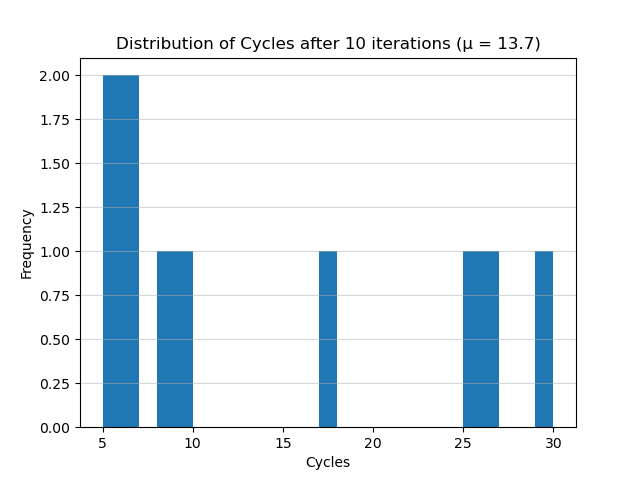
\includegraphics[width=\textwidth]{10.png}
  \caption{10 games}
  \label{fig:10}
\end{subfigure}%
\begin{subfigure}{.5\textwidth}
  \centering
  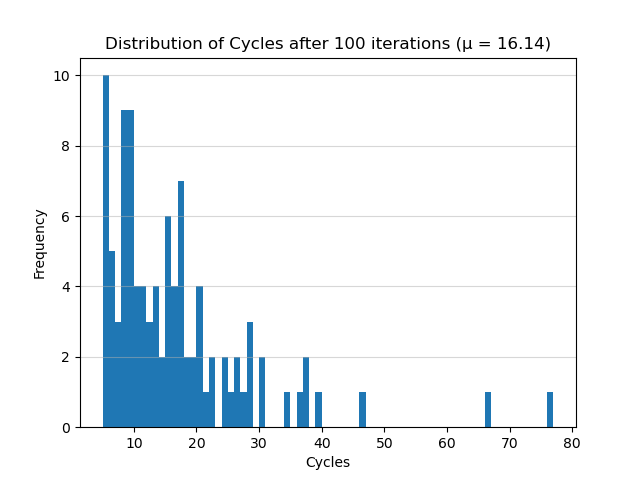
\includegraphics[width=\textwidth]{100.png}
  \caption{100 games}
\end{subfigure}
\caption{Plots of the distribution of cycles after simulating various numbers of games}
\label{fig:dist}
\end{figure}

\begin{figure}[H]
\centering
\begin{subfigure}{.5\textwidth}
  \centering
  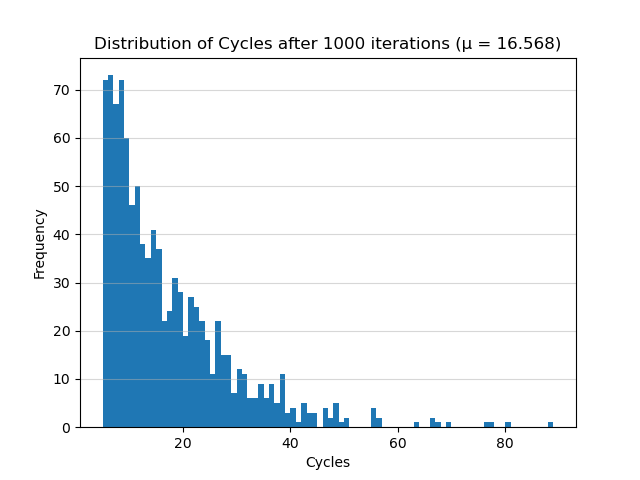
\includegraphics[width=\textwidth]{1000.png}
  \caption{1000 games}
\end{subfigure}%
\begin{subfigure}{.5\textwidth}
  \centering
  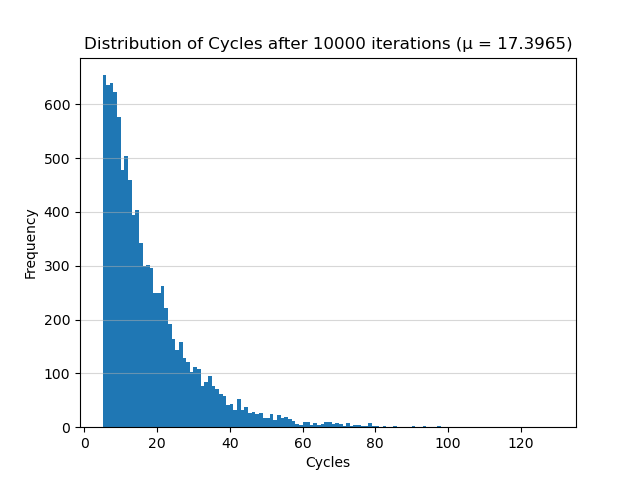
\includegraphics[width=\textwidth]{10000.png}
  \caption{10000 games}
  \label{fig:10000}
\end{subfigure}
\caption{Plots of the distribution of cycles after simulating various numbers of games}
\label{fig:dist}
\end{figure}

\begin{figure}[H]
\centering
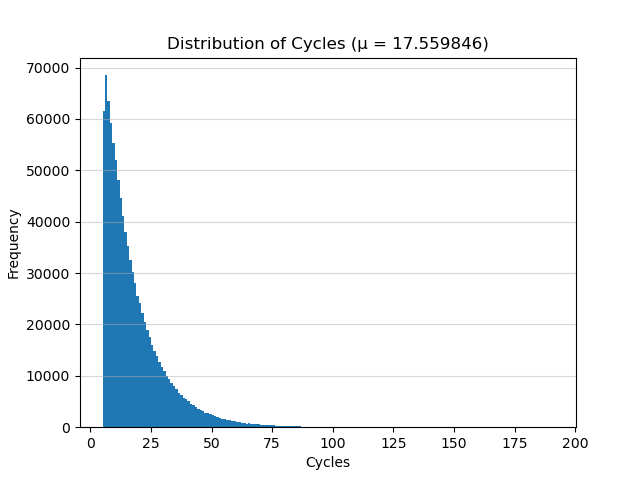
\includegraphics[width=.75\textwidth]{1000000.png}
\caption{Plots of the distribution of cycles after simulating 1,000,000 games}
\label{fig:1000000}
\end{figure}

It can be noted from these figures that the lowest number of cycles is 5 cycles. This is intuitive, since the players start with 4 coins, and would have to roll a 4, 5, or 6 five times in a row to lose the game in the least number of rolls. It can also be seen that the distribution of cycles becomes highly right-skewed as the number of games played increases. It is also worth noting that although the distribution looks like an exponential distribution, that is not so, as a property of the exponential distribution is that it is constantly decreasing, whereas it can be seen in Figure \ref{fig:1000000} that the frequency of `5 cycles' is lower than `6 cycles'.

To find the expected value of the distribution, the mean of the distribution of cycles was found. The movement of the mean over 1,000,000 games can be seen in Figure \ref{fig:mean}. It can be seen in this plot that the mean of the distribution eventually balances around 17.5603 cycles.

\begin{figure}[H]
\centering
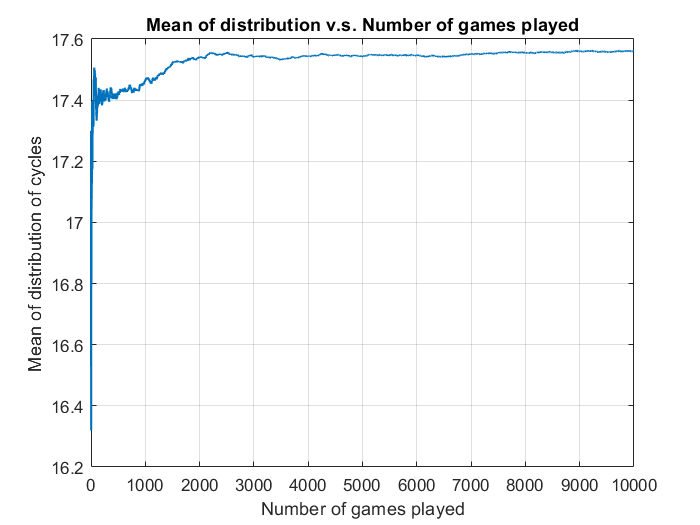
\includegraphics[width=.75\textwidth]{mean.png}
\caption{Mean of the distribution of cycles over 1,000,000 simulations}
\label{fig:mean}
\end{figure}